

\documentclass[]{article}

\usepackage[margin=1in]{geometry}

\usepackage[]{amsthm}
\usepackage[parfill]{parskip}
\usepackage[]{graphicx}
\graphicspath{{../img/}}

\newtheorem{theorem}{Theorem}
\newtheorem{lemma}{Lemma}
\newtheorem{corollary}[]{Corollary}

\title{CMSC 510: Single Shortest Path Algorithms --- Pseudocode}
\author{Acacia Ackles}

\begin{document}

\maketitle

\section*{Introduction}

We're now continuing our theme of looking at graphs and ways to traverse graphs. 

Up until now we've been considering a few different ways to look for minimal paths from some node, starting with Breadth-First Search which looked at shortest paths from some source node in terms of the number of edges to traverse. 

Then we looked at graphs with weighted edges, where we had to consider the value of each edge we were adding, and how to get to every node in the graph with the minimal total graph weight. 

The next natural thing to do might be to combine both those ideas. What if we want the shortest path in terms of weight from one particular node to another particular node? What kind of algorithm might we want then? 

\section*{General Concepts for Shortest-Path Algorithms}

\subsection*{Problem Statement}

A common way to think about this problem is the literal shortest path between two points, as in a GPS. How might we be able to generalize Breadth First Search to address this kind of problem? 

\subsection*{Cycles}

There are a few things we might need to consider for a general algorithm about shortest-paths that we didn't have to consider in this problem statement, because of its connection to a real-world example. These kinds of ``edge cases'' are common considerations when designing a real algorithm from scratch. 

In particular, we need to be conscious of \textit{cycles}. 

What about a positive-weight cycle? Removing such a cycle would actually shorten the graph, so we'd never want a positive-weight cycle. 

A 0-weight cycle? Technically, yes, this would still be a valid shortest path, but we can always replace this path with one of identical weight that is not a cycle without losing anything about the graph. So for simplicity's sake, we can ignore the existence of 0-weight cycles.

Shortest paths, therefore, can be assumed to be simple paths: paths with no cycles. 

In our case we're going to look at single-source shortest paths, which are paths from a chosen single vertex to any other vertex in the graph. 

\subsection*{Initialization}

First we want to start our search with some kind of initial condition for each vertex other than our source vertex. This will look much like our initialization for BFS and DFS.  

\begin{figure}[h]
    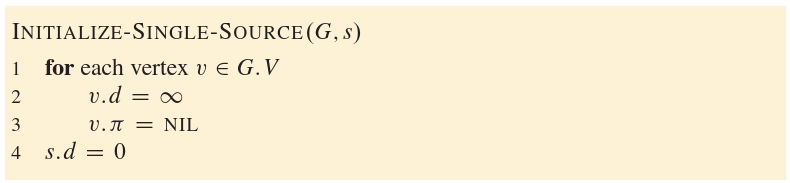
\includegraphics[width=\textwidth]{ssp-initialize-pseudo.png}
\end{figure}

Now, since the distance to every vertex is set to positive infinity, whenever we traverse the graph and find an edge to that vertex, we'll want to update our understanding of what the shortest path to that graph is. 

In mathematical terms, for two vertices $u$ and $v$, if $v.d \leq u.d + w(u,v)$, then we update $v.d$ to be $u.d + w(u,v)$. This procedure is calld ``relaxation'', even though it is a tightening of a bound. The reasoning has to do with historical terminology. 

The relaxation pseudocode itself is quite simple:

\begin{figure}[h]
    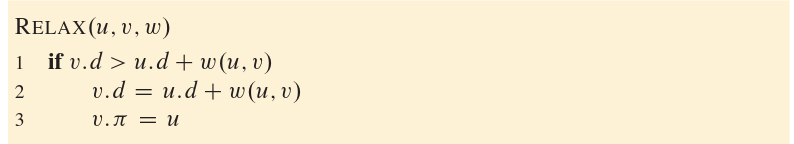
\includegraphics[width=\textwidth]{ssp-relax-pseudo.png}
\end{figure}

So now that we know how to initialize a graph, and how to update edges when we find a shorter path, we can turn back to our algorithm attempts for finding shortest paths. 

Knowing now that every time you find a shorter path between two vertices you will perform some sort of relaxation procedure, take a few more minutes to discuss how you'd create a shortest path algorithm. 

\section*{Dijkstra's Algorithm}

Let's first consider a generalization of the Breadth-First Search algorithm we've become familiar with. Like with BFS, we want to expand outward in our search as a ``wave'', and as we hit each successive point, we consider the edges at those points. 

In BFS, we would then put the next edge to consider at the back of a first-in first-out (FIFO) queue.

Where might we run into problems with this approach? 

Well, the purpose of the FIFO queue in BFS is to choose the next vertex from which to send out an edge. That is, it is to choose the next closest vertex to the source. In that case we only need to store a single piece of information about the vertex: when we encountered it. They are sorted as such.

Now, we need a different data structure which will somehow sort the vertices not by the time we found it, but by the path length to that vertex. 

Have we already seen an algorithm which does something like this? i.e., selecting the cheapest edge? 

In this case we're using a min-priority queue, $Q$, so we can extract the minimum easily. 

We then maintain a set of ``finished'' vertices, $S$. As a vertex is added to the set, all edges leaving that vertex are relaxed. The next vertex to add is determined by the minimum in the priority queue. 


\begin{figure}[h]
    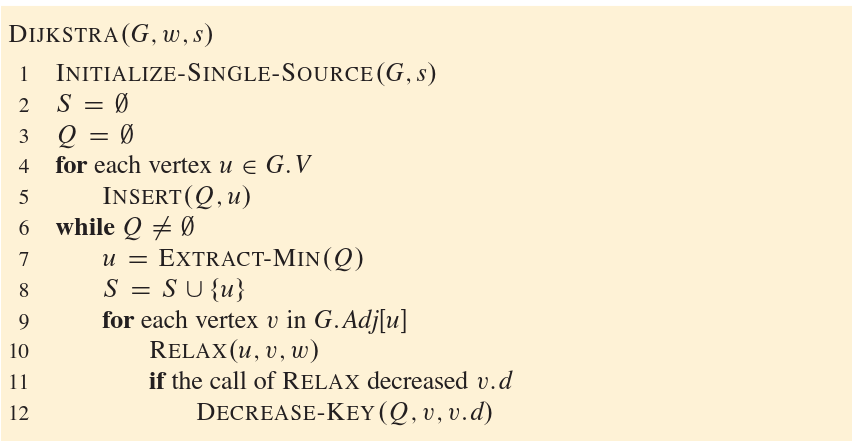
\includegraphics[width=\textwidth]{djikstra-pseudo.png}
\end{figure}

\begin{figure}[h!]
    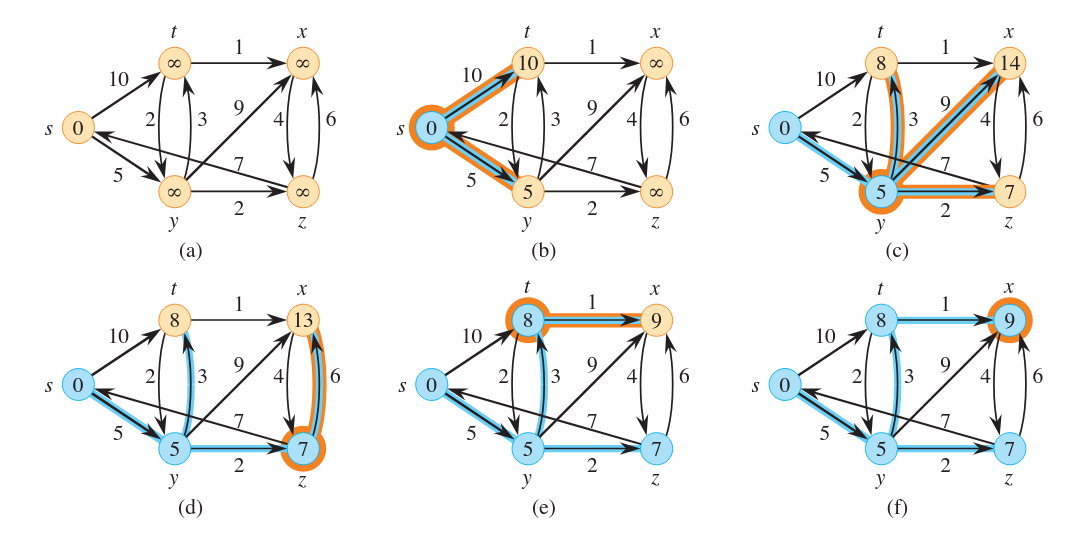
\includegraphics[width=\textwidth]{djikstra.png}
\end{figure}


\section*{Algorithms for Negative-Weight Edges}

Recently, Google Maps has implemented an ``energy-efficient'' route option when you pull up directions on the GPS. Ignoring the fact that the true most ``energy-efficient'' route is to build a functioning public transit system in America, let's consider one aspect of these routes.

For hybrid or electric cars, going uphill or on a slope takes energy, while going downhill generates energy. This means if we want to consider only the energy associated with a given route, some of our weights will be negative, while some will be positive. I'll draw an example in class, but there is one in your book as well.

You are trying to find the most energy-efficient route from your house to your work given some graph of intersections and weights (positive or negative) between those intersections. 

Will Dijkstra's algorithm still work here?

What considerations would you have to make for an algorithm that can accomplish this task?

\subsection*{Cycles}

Could we include a negative-weight cycle in our shortest path? That would probably be bad, because then we'd just spiral down into infinitely short paths, which isn't really in the spirit of what we are trying to find. 

\section*{Bellman-Ford Algorithm}

For this case, we need the Bellman-Ford Algorithm. This algorithm doesn't specifically select a vertex to start from every time; it just checks every edge for as many vertices as there are other than the source.


\begin{figure}[h]
    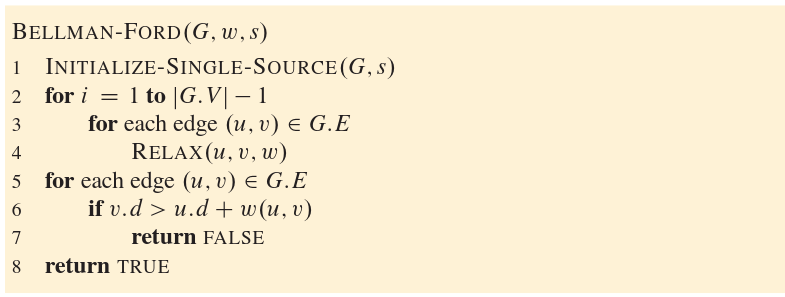
\includegraphics[width=\textwidth]{ssp-bellman-ford-pseudo.png}
\end{figure}

\begin{figure}[h]
    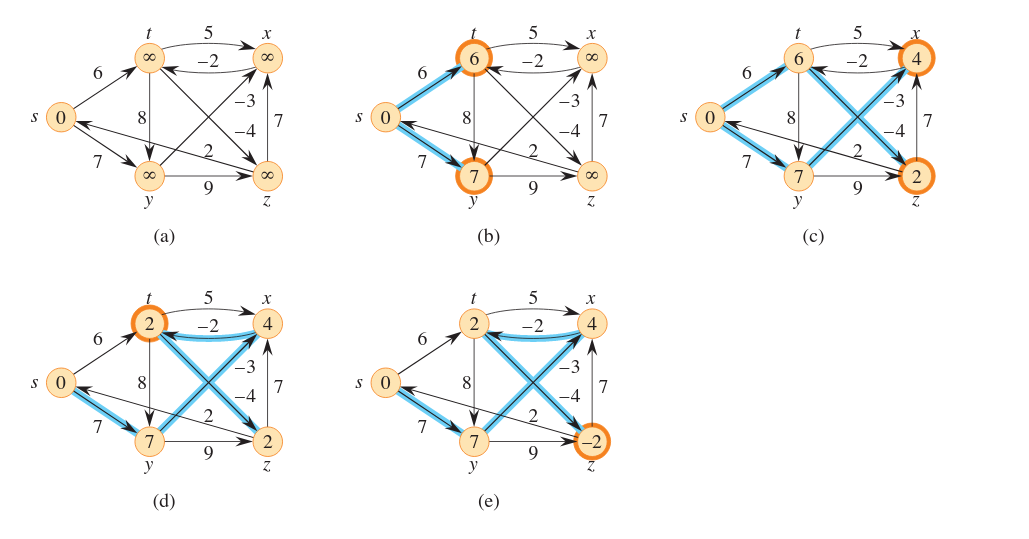
\includegraphics[width=\textwidth]{ssp-bellman-ford.png}
\end{figure}

Note that it is \textit{not choosing a vertex} each time it runs. The reason $x$ and $z$ vertices don't get updated here is not because they haven't been considered. It's because when they were considered, the distance between $t$ and $x$ was infinity plus infinity, so no update was performed. That is not clear from the picture, but the figure caption in the book shows it. 

As you might imagine, an algorithm that runs on every edge for every vertex is not a particularly efficient algorithm, but it is one that is equipped to handle negative weights. 

\end{document}
